\documentclass{article}


\usepackage{listings}
\usepackage{xcolor}
% Language setting
% Replace `english' with e.g. `spanish' to change the document language
\usepackage[english]{babel}

% Set page size and margins
% Replace `letterpaper' with `a4paper' for UK/EU standard size
% \usepackage[a4paper,top=1.5cm,bottom=1.7cm,left=1cm,right=1cm,marginparwidth=1.75cm]{geometry}
\usepackage[a4paper, margin=0.72in]{geometry}

% Useful packages
\usepackage{amsmath}
\usepackage{graphicx}
\usepackage[colorlinks=true, allcolors=blue]{hyperref}

\title{COL216 Semester 2024-25 Sem II Assignment - 3}

\author{
    Aadi Govil (2023CS10490) |
    Apurva Samota (2023CS10585)
}


\begin{document}

\maketitle

\section{Assumptions:}
\begin{enumerate}
    \item LRU cache - cache line eviction is based on LRU i.e. least-recently used 
    \item Transaction arbitration is being done according to the lowest index.
    \item To halt a core on writeback/transfer for another core, we have added a toggler so we can run both by changing one global variable - \texttt{IF\_EVICT\_OR\_TRANSFER\_STALL}.
    \item There can be only one active bus transaction at a time - either writeback/transfer or invalidate.
    \item Checking neighbors in bus transactions is considered almost instantaneous, i.e. one can check neighbors \& get started on data transfer in the same cycle.
    \item Per cycle, only one processing can be done on bus.
    \item If there is miss at cycle T : then it will get back data in cycle T+100 \& performs hit on data in the same cycle.
\end{enumerate}

\section{Definitions:}
\begin{enumerate}
    \item Execution Cycles: Cycles in which either it computes an instruction or the bus is doing something to help compute its instruction. These may include write-backs. This is only till PC is less than no. of instructions for the respective core.
    \item Idle Cycles: All Cycles that occur before PC exceed the size of the instructions vector but which are not counted in the execution cycles.
    \item Misses: This can be at most one per instruction.
    \item Cache evictions: When M/E/S block becomes I.
    \item Writeback: When M block becomes I.
    \item Invalidations: Any \texttt{RdX} or Invalidate signal that a core sends out to the bus.
    \item Data Traffic: Any input/output cacheline going in/out of the core.
    \item Bus Traffic: This includes any cachelines transferred to the bus for any transaction: memory to cache, cache to cache, or writebacks.
    
\end{enumerate}


\section{Implementation Details:}
\subsection{Main Classes:}
\begin{enumerate}
    \item \texttt{cacheLine}: Represents a single cache block. Stores tag, state,(eg. Modified, Shared, Exclusive, Invalid), and line size bits.
    \item \texttt{cacheSet}: Contains multiple \texttt{cacheLine} entries. Supports tag lookup and LRU-based replacement. Maintains an LRU list using a doubly-linked list.
    \item \texttt{cache}: Represents a single cache core. Stores \texttt{cacheSet} entries and processes memory read/write instructions. Handles cache hit/miss detection, MESI  state transitions, and bus requests.
    \item \texttt{bus}: Simulates a shared bus across quad cores. Handles arbutration, memory fetches, invalidations, and updates during \texttt{Rd}/\texttt{RdX}/\texttt{WriteInvalidate} transactions.
\end{enumerate}






\subsection{Data Structures Used:}
\begin{enumerate}
    \item \texttt{std::vector}: Used to store: instructions, cache lines within set, sets within each cache.
\end{enumerate}




\section{Flow-Chart for functions:}
\subsection{\texttt{bus::runForACycle}} : 
\begin{figure}[h]
  \centering
  \includegraphics[width=0.7\textwidth]{Screenshot 2025-04-30 221603.png}
  \caption{\texttt{bus::runForACycle} work-flow}
  \label{fig:arch}
\end{figure}
\subsection{\texttt{cache::processSnoop}} :
\begin{figure}[h]
  \centering
  \includegraphics[width=0.7\textwidth]{Screenshot 2025-04-30 221613.png}
  \caption{\texttt{cache::processSnoop} work-flow}
  \label{fig:arch}
\end{figure}
\subsection{\texttt{cache::processInst}} :
\begin{figure}[h]
  \centering
  \includegraphics[width=0.7\textwidth]{Screenshot 2025-04-30 222507.png}
  \caption{\texttt{cache::processInst} work-flow}
  \label{fig:arch}
\end{figure}
\section{Experiments:}
\subsection{Varying associativity:}
We fixed setBits at 6 and lineSizeBits at 5 and varied associativity E from 1,2,4,8,16 which lead to the following results from app1:
\begin{figure}[h]
  \centering
  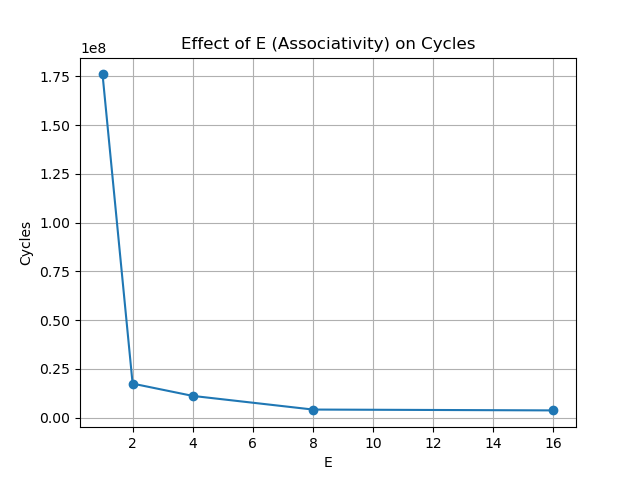
\includegraphics[width=0.7\textwidth]{plot_vary_E.png}
  \caption{Varying associativity}
  \label{fig:arch}
\end{figure}
This result is obtained because you can store more cache lines that map to the same set as the associativity decreases, which helps improve time by reducing the number of cache write backs to the memory and improving the number of cache hits.

\subsection{Varying number of sets per cache:}
We fixed associativity at 2 and lineSizeBits at 5 and varied setBits from 1 to 6 which lead to the following results from app1:
\begin{figure}[h]
  \centering
  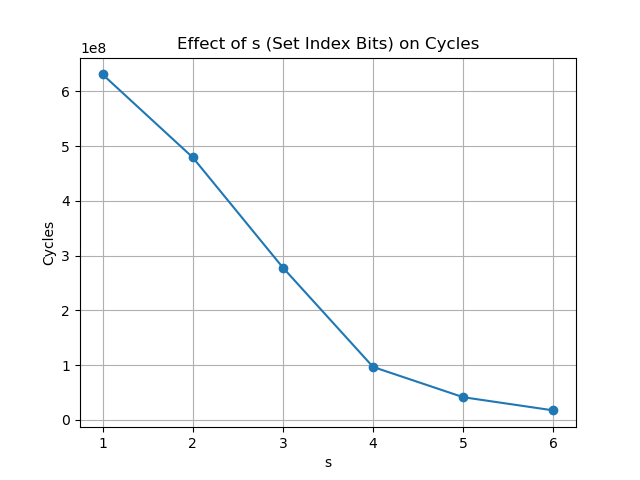
\includegraphics[width=0.7\textwidth]{plot_vary_s.png}
  \caption{Varying set bits}
  \label{fig:arch}
\end{figure}
As the associativity for the cache is very small so for small values of set bits, the amount of space available to the cache is very small. Moreover, more is the amount of set bits, more is the amount of sets, and hence lower is the false sharing, which helps reduce the amount of invalidates between 2 caches as well as evictions within the same cache.

\subsection{Varying number of bytes per cache line:}
We fixed associativity at 2 and setSizeBits at 6 and varied setBits from 2 to 6 which lead to the following results from app1:
\begin{figure}[h]
  \centering
  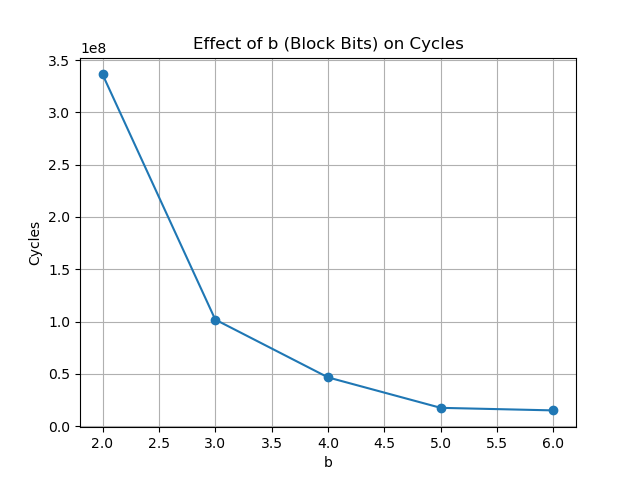
\includegraphics[width=0.7\textwidth]{plot_vary_b.png}
  \caption{Varying set bits}
  \label{fig:arch}
\end{figure}
As the amount of bits per cache line increase, the locality of running program gets better, i.e, if I got hit on me and then my neighbouring word is called down the line, I would not hit in case the number of set bits is lesser, but would hit if the number of set bits is higher. This causes an decrease in the amount of cycles taken for me to run the program app1.


\section{Interesting hand generated trace}

We have added a trace test to the submission. What is interesting about this trace? 

This trace is a small trace which gives different outputs for both the versions of our assignment submissions, even though running for the same amount of cycles.

Secondly it features false sharing heavily, and we can see its effects.

Thirdly we can see the graph given by it on varying the number of bytes per cache line which is very interesting to see as well.











\end{document}
